\chapter{Literature review}
\label{chap:literature_review}

Longitudinal causal inference is a broad area of research with a rich literature. There are 
two main dimensions along which the literature can be organized. The first is the structure 
of the causal setting, typically represented by a directed acyclic graph (DAG) 
with a set of nodes $\mathbf{V}$ and a set of directed edges $\mathbf{E}$. 
Each node in the graph represents a variable and each directed edge 
represents a causal relationship between two variables. 
The structure of the causal diagram encodes the assumptions about the 
data generating process and the causal relationships between the variables \cite{pearlCausalityModelsReasoning2009}. This includes 
features such as the presence or absence of treatment-confounder feedback or presence 
of unobserved confounders as shown in Figure \ref{fig:sample_dags}.

The second dimension is about the causal target of interest, that is, the 
estimand addressed by the method. This dimension is driven by the research question and 
the scientific context of the study \cite{lundbergWhatYourEstimand2021}. 
For example, in a longitudinal study with time-varying treatments, 
one might be interested in estimating the average treatment effect at a specific time point, 
the cumulative effect of the treatment over time, or the effect of a specific treatment regime. These 
targets are often formalized in the potential-outcomes framework, which is introduced in 
detail in Chapter ~\ref{chap:method}.




\begin{figure}[htbp]
\centering

\begin{subfigure}{0.9\textwidth}
\centering
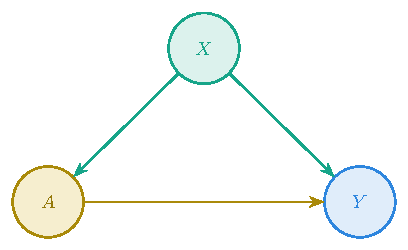
\includegraphics[width=\linewidth]{figures/build/simple_dag.pdf}
\caption{A simple causal DAG with treatment $A$, outcome $Y$, and confounder $X$. The confounder $X$ is a common cause of both the treatment $A$ and the outcome $Y$, which can lead to confounding bias if not properly adjusted for.}
\end{subfigure}

\vspace{0.6cm}

\begin{subfigure}{0.9\textwidth}
\centering
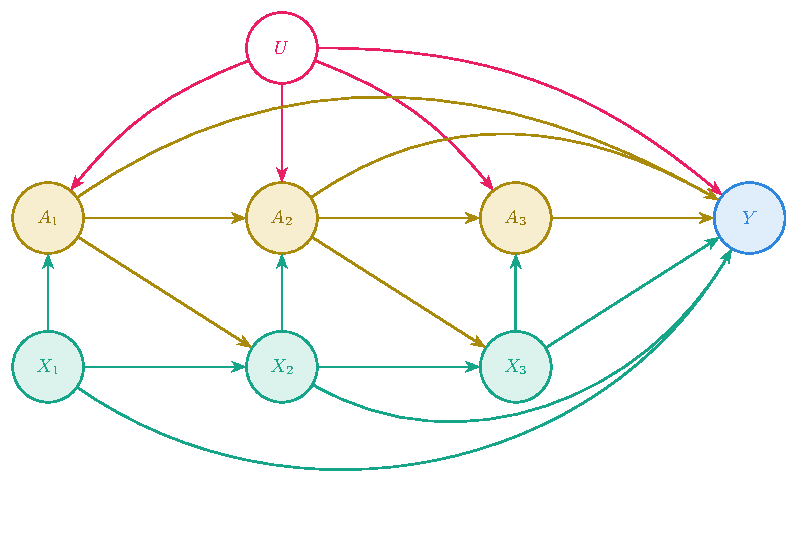
\includegraphics[width=\linewidth]{figures/build/treatment_covariate_feedback.pdf}
\caption{A longitudinal causal DAG with time-varying treatments $A_t$, time-varying confounders $X_t$, and an unobserved confounder $U$.
Filled nodes represent observed variables, while the unfilled node represents an unobserved variable. Arrows 
from $A_t$ to $X_{t+1}$ represent treatment-confounder feedback, where the treatment at time $t$ can affect the confounders at later time points.}
\end{subfigure}

\caption{Two examples of causal DAGs. The first DAG (a) represents a simple static setting with a single treatment and outcome, while the second DAG (b) represents a more complex longitudinal setting with time-varying treatments.}
\label{fig:sample_dags}
\end{figure}

 

and the second dimension is the presence or absence of such feedbacks.
To situate the two methods that we are going to compare in this thesis, we will review 
There are different suggested identification strategies for specifically designed to address such feedbacks such as the g-formula or inverse probability of treatment weighting (IPTW) \cite{robinsEstimationCausalEffects2008a}. 
However, these identification strategies rely on the assumption of 
sequential ignorability, which states that the researcher 
has gathered all the \emph{required} data for the causal analysis or more  
formally there are no unmeasured confounders between the treatments and the outcome at each time point. %In the most general case, 
%confounders can be seen as a common cause of two or more variables in the causal graph. 
%In the context of longitudinal data, we are often concerned about unmeasured confounders effecting the 
%treatment assignment and the outcome at each time point.  
This is a strong assumption and often violated in real world settings. 

To address the problem of unmeasured confoundedness in static settings, there have been 
different methods proposed. Some need additional data with a very specific 
structure such as instrumental variable methods \cite{angristIdentificationLocalAverage1996} 
or using proxy variables \cite{tchetgenIntroductionProximalCausal2020}, 

while others rely on strong assumptions about the data generating process such as the deconfounder method \cite{wangBlessingsMultipleCauses2019}.